\section{Prototipo y resultados preliminares}\label{sec:resultados}

\subsection{Prototipo}
\textbf{Repositorio:} \colorbox{yellow}{[completar con la URL de GitHub del grupo]}

\begin{lstlisting}
transporte-cusco-scheduling/
|-- src/bus_sched/     traffic · model · builder · validator · metrics · viz · cli
|   `-- algorithms/    greedy.py (LS, LPT) · bnb.py, cpsat.py (referencia, etapa posterior)
|-- tests/             pytest: test_ls_lpt · test_traffic · test_datos · test_referencia
|-- experiments/       run_experiments.py (E1) · build_excel.py · export_latex.py · demo_prototipo.ipynb
|-- data/              raw/ (Excel, 35 rutas) · instances/ (JSON) · traffic/ (perfiles JSON)
|-- results/           E1_35_rutas.csv · E1_resumen.csv · figuras · Excel de la entrega
`-- docs/              informe LaTeX, plan de aprendizaje, bitácoras, contribuciones
\end{lstlisting}

El prototipo \textbf{carga una instancia, genera las vueltas, ejecuta LS o LPT, valida la solución y produce una salida verificable}. Las capturas siguientes corresponden a la ejecución en el equipo del grupo (Windows, PowerShell, entorno virtual \texttt{.venv}).

\textbf{Construcción de instancias y perfiles.} El comando \texttt{build} lee el Excel del proyecto, genera las vueltas de las 35 rutas con la regla general, verifica que coincidan con la hoja \emph{Trabajos y ventanas} y escribe las instancias JSON y los perfiles de tráfico. El comando \texttt{profiles} muestra los tres escenarios: T1 tiene media ponderada 1.000 en la jornada y T2, 1.128.

\captura{build_instancias.png}{Generación de las 35 instancias y de la instancia DEMO (\texttt{python -m bus\_sched build}).}{fig:cap-build}

\captura[0.8\textwidth]{cli_profiles.png}{Perfiles de tráfico T0, T1 y T2 (\texttt{python -m bus\_sched profiles}).}{fig:cap-profiles}

\textbf{Ejecución sobre una ruta real.} La ruta RTI-01 (E.T. Saylla S.A., 35 buses, 103 vueltas) se resolvió con ambos algoritmos en los tres escenarios. Cada ejecución imprime las métricas, valida la solución y guarda las asignaciones en \texttt{results/RTI-01\_<alg>\_<tráfico>.csv}. La tabla~\ref{tab:rti01} resume las seis ejecuciones; los valores coinciden con las filas de RTI-01 en \texttt{results/E1\_35\_rutas.csv}.

\begin{table}[H]
\centering\small
\caption{Ejecuciones de LS y LPT sobre RTI-01 (103 vueltas, 35 buses).}\label{tab:rti01}
\begin{tabular}{llrrrrrc}
\toprule
Tráfico & Algoritmo & Atendidas & \makecell{$\Lmax$\\(h)} & \makecell{Cota\\inferior (h)} & \makecell{Brecha\\vs $LB$} & \makecell{Desbalance\\(h)} & Validación \\
\midrule
T0 & LS = LPT & 103/103 & 7.440 & 7.298 & 1.9\,\% & 2.480 & OK \\
\midrule
T1 & \textbf{LS} & \textbf{103/103} & \textbf{7.772} & 7.063 & \textbf{10.0\,\%} & \textbf{2.565} & OK \\
T1 & LPT & 100/103 & 9.733 & 6.875 & 41.6\,\% & 4.629 & OK \\
\midrule
T2 & \textbf{LS} & \textbf{99/103} & \textbf{8.625} & 7.621 & \textbf{13.2\,\%} & \textbf{2.885} & OK \\
T2 & LPT & 90/103 & 10.852 & 7.021 & 54.6\,\% & 5.117 & OK \\
\bottomrule
\end{tabular}
\end{table}

\captura{run_ls_RTI-01_T1.png}{List Scheduling sobre RTI-01 con tráfico T1 y diagrama de Gantt (\texttt{--gantt}).}{fig:cap-ls}

\captura{run_lpt_RTI-01_T1.png}{LPT sobre RTI-01 con tráfico T1.}{fig:cap-lpt}

\captura{run_ls_RTI-01_T0.png}{List Scheduling sobre RTI-01 sin tráfico (T0).}{fig:cap-ls-t0}

\captura{run_ls_RTI-01_T2.png}{List Scheduling sobre RTI-01 con el perfil pesimista T2.}{fig:cap-ls-t2}

\captura{run_lpt_RTI-01_T0_T2.png}{LPT sobre RTI-01 sin tráfico (T0) y con el perfil pesimista T2.}{fig:cap-lpt-t0t2}

Sin tráfico ambos algoritmos producen la misma solución. Con T1, LS atiende las 103 vueltas con $\Lmax = 7.772$\,h, mientras que LPT deja 3 sin atender y llega a 9.733\,h; con T2 la diferencia crece (4 frente a 13 vueltas no atendidas). Todas las soluciones pasan el validador sin violaciones, y cada ejecución tarda entre 20 y 31\,ms.

Una instancia conocida (la de la sección~\ref{sec:manual}) o una nueva escrita en el formato JSON de la sección~\ref{sec:sistema} se resuelve con \texttt{python -m bus\_sched run --instance archivo.json --alg ls} (o \texttt{--alg lpt}), y el validador confirma su factibilidad.

\begin{figure}[H]
\centering
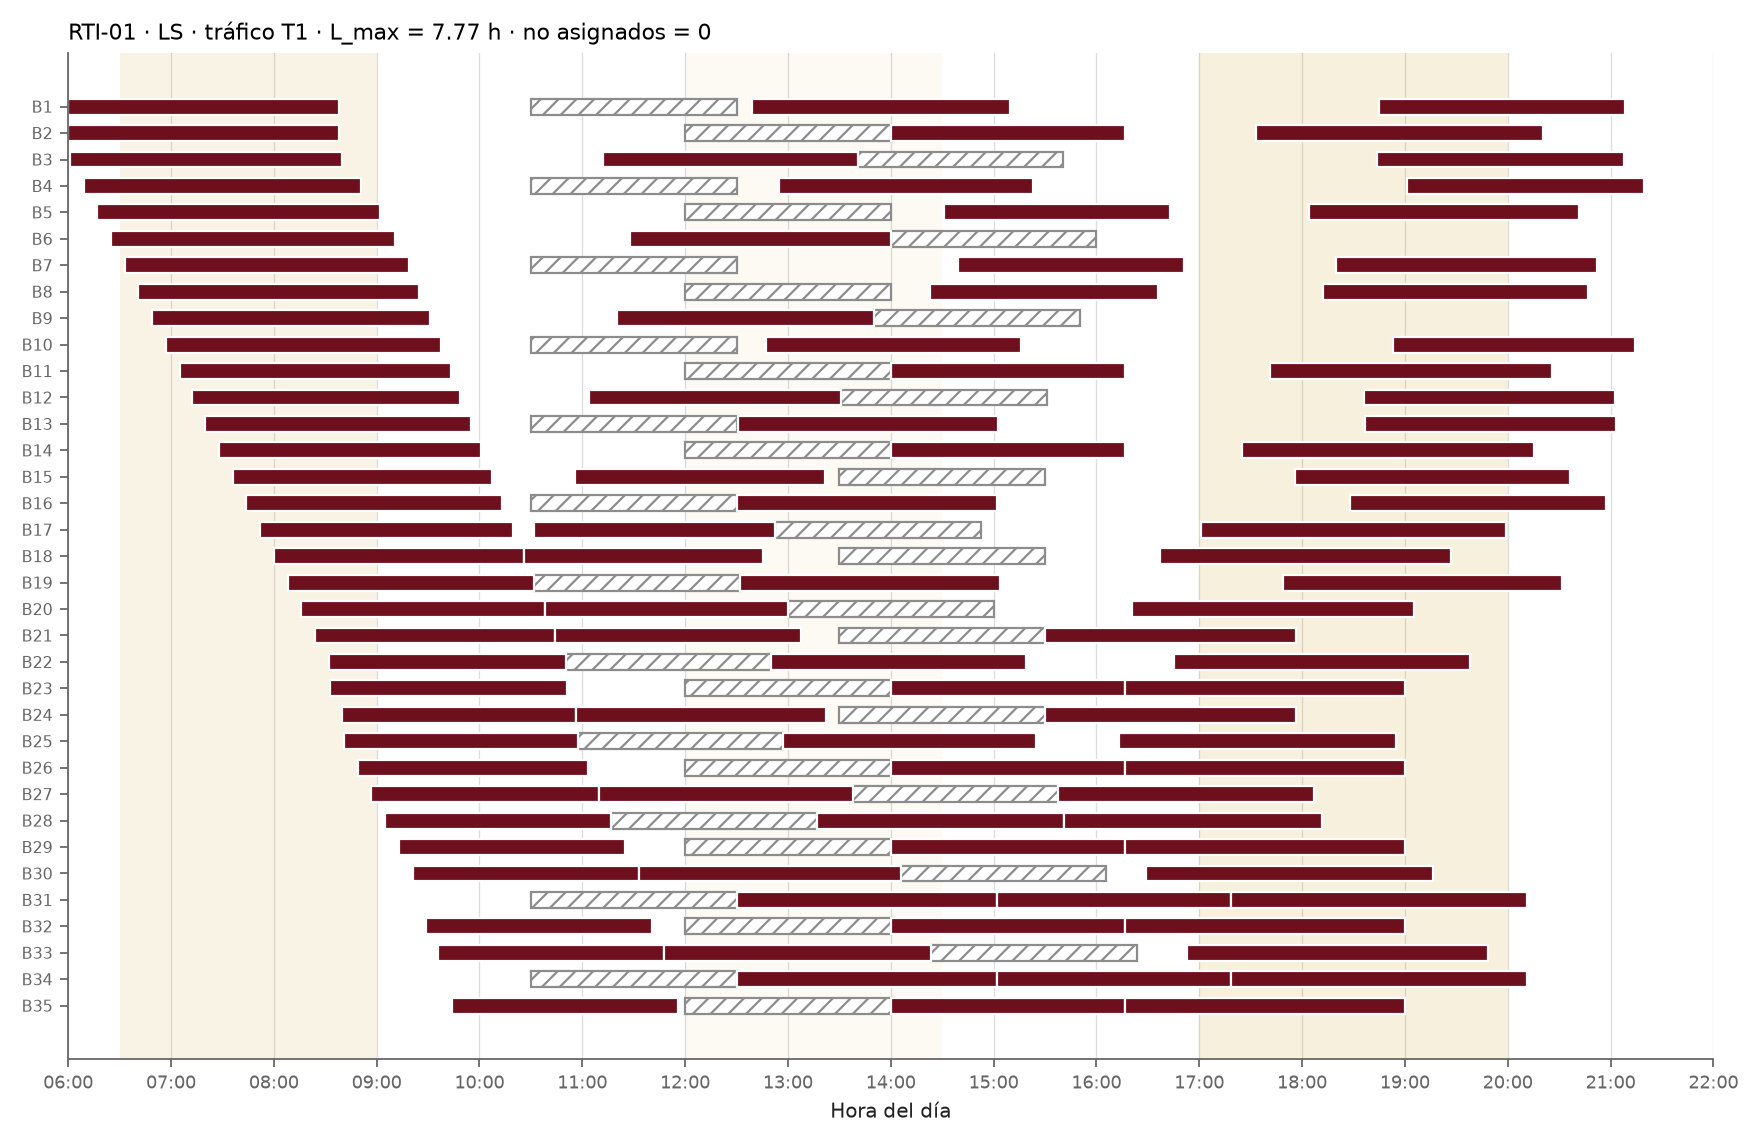
\includegraphics[width=0.95\textwidth]{figuras/fig_gantt_RTI-01_LS_T1.png}
\caption{Programa de RTI-01 (35 buses, 103 vueltas) con List Scheduling y tráfico T1.}\label{fig:gantt-rti01}
\end{figure}

\subsection{Resultados preliminares de E1}\label{sec:e1}
\begin{table}[H]
\centering\small
\caption{Resultados agregados de E1 sobre las 35 rutas (4\,733 vueltas; brecha y desbalance promediados por ruta; 0 violaciones en todas las soluciones).}
\label{tab:e1}
\begin{tabular}{llrrrrrr}
\toprule
Tráfico & Algoritmo & No atendidas & \makecell{Rutas\\completas} & \makecell{$L_{\max}$\\medio (h)} & \makecell{Brecha\\vs $LB$} & \makecell{Desbalance\\(h)} & \makecell{Sobrecosto\\por tráfico} \\
\midrule
T0 & LS = LPT & 87 (1.8\,\%) & 18 & 9.15 & 10.3\,\% & 1.91 & 0.0\,\% \\
\midrule
T1 & \textbf{LS} & \textbf{155 (3.3\,\%)} & 8 & \textbf{8.96} & \textbf{13.6\,\%} & \textbf{1.65} & +0.8\,\% \\
T1 & LPT & 293 (6.2\,\%) & 10 & 9.13 & 19.4\,\% & 2.53 & +0.8\,\% \\
\midrule
T2 & \textbf{LS} & \textbf{255 (5.4\,\%)} & 4 & \textbf{9.87} & \textbf{14.2\,\%} & \textbf{1.92} & +13.4\,\% \\
T2 & LPT & 547 (11.6\,\%) & 4 & 10.04 & 24.1\,\% & 3.41 & +13.7\,\% \\
\bottomrule
\end{tabular}
\end{table}


\begin{figure}[H]
\centering
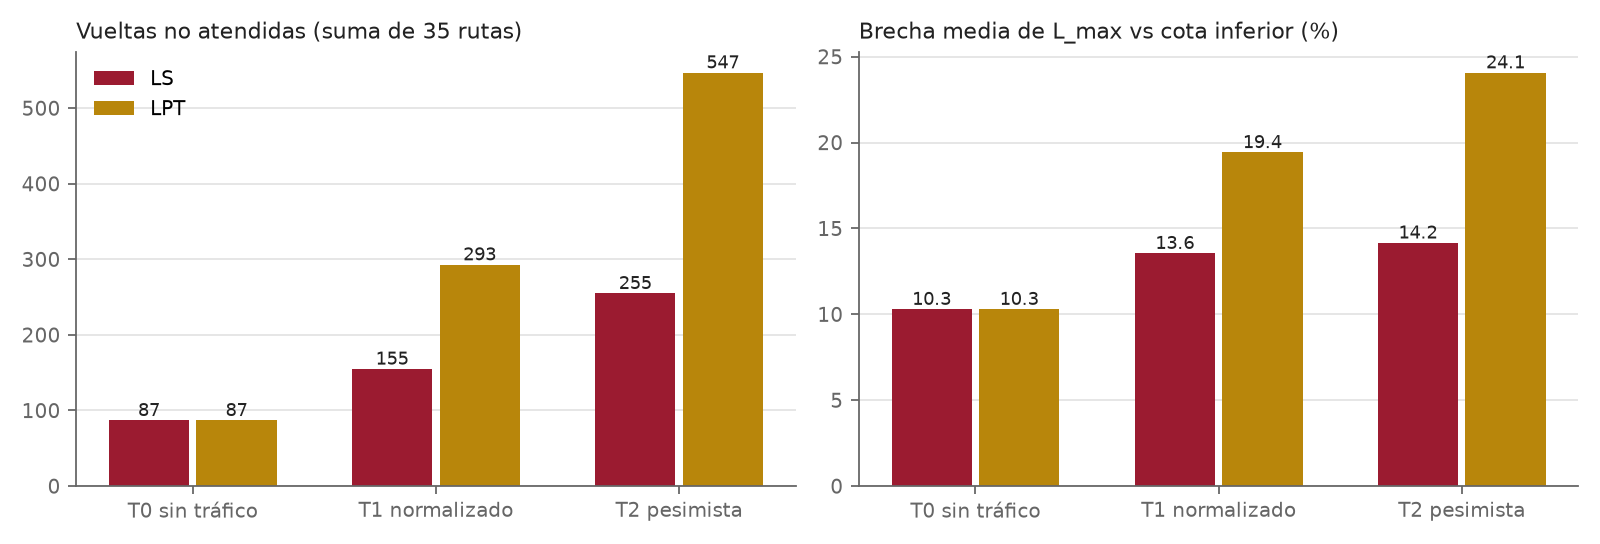
\includegraphics[width=\textwidth]{figuras/fig_E1_escenarios.png}
\caption{Vueltas no atendidas y brecha media respecto de la cota inferior, por escenario de tráfico.}\label{fig:e1}
\end{figure}

El experimento se ejecuta con \texttt{python experiments/run\_experiments.py}, que resuelve las 35 rutas con LS y LPT en T0, T1 y T2, valida cada solución y escribe \texttt{results/E1\_35\_rutas.csv} (una fila por ruta, algoritmo y escenario) y el resumen \texttt{results/E1\_resumen.csv}. Después, el script \texttt{build\_excel.py} de \texttt{experiments/} vuelca esos resultados en el Excel de la entrega.

\captura{run_experiments_E1.png}{Ejecución del experimento E1 (\texttt{python experiments/run\_experiments.py}); el proceso completo terminó en 9\,s.}{fig:cap-e1}

\captura{E1_resumen_csv.png}{Contenido de \texttt{results/E1\_resumen.csv}, origen de la tabla~\ref{tab:e1}.}{fig:cap-e1-resumen}

\captura[0.8\textwidth]{E1_archivos.png}{Archivos de resultados de E1 generados en \texttt{results/}.}{fig:cap-e1-archivos}

\captura[0.85\textwidth]{build_excel.png}{Generación del Excel de la entrega (\texttt{python experiments/build\_excel.py}).}{fig:cap-build-excel}

\begin{itemize}
  \item \textbf{Sin tráfico, LS y LPT coinciden.} Las vueltas de una ruta tienen la misma duración base, así que el orden de LPT empata y se desempata por $r_j$, que es el orden de LS.
  \item \textbf{Con tráfico, LS obtiene mejores resultados en las instancias evaluadas.} En T1 deja 155 vueltas sin atender frente a 293 de LPT y es igual o mejor en 26 de 35 rutas; en T2 es mejor en 31 de 35. Su desbalance es 35--44\,\% menor.
  \item \textbf{El tráfico reduce la atención:} con LS, la proporción de vueltas atendidas pasa de 98.2\,\% (T0) a 96.7\,\% (T1) y 94.6\,\% (T2). En T1 la conducción total casi no cambia (+0.8\,\%), porque el perfil solo redistribuye el tiempo; en T2 aumenta 13.4\,\%.
  \item \textbf{Las vueltas no atendidas sin tráfico se concentran en rutas saturadas:} RTU-22 (21; $\rho = 1.02$), RTI-02 (15; $\rho = 0.87$), RTU-01 (12; $\rho = 0.79$) y RTU-05 (7; $\rho = 0.82$).
  \item \textbf{Tiempo de ejecución:} en el equipo del grupo, cada configuración (algoritmo y escenario) resolvió las 35 rutas en 0.84--1.03\,s, es decir, entre 24 y 30\,ms por ruta en promedio.
\end{itemize}

\subsection{Contraste con las hipótesis}
\begin{table}[H]
\centering\small
\caption{Contraste preliminar de hipótesis.}
\begin{tabularx}{\textwidth}{L{4.8cm}YL{3.0cm}}
\toprule
Hipótesis & Resultado preliminar & Estado \\
\midrule
H1: LS = LPT sin tráfico; LS mejor con tráfico & Idénticos en T0; LS mejor en T1 y T2 & Se cumple en las instancias evaluadas \\
H2: efecto moderado de T1 y marcado de T2 & +68 vueltas no atendidas en T1 (+1.4\,pp) y +168 en T2 (+3.5\,pp) respecto de T0 & Se cumple \\
H3: no atendidas concentradas en rutas de alta $\rho$ & Las 4 rutas con más vueltas no atendidas tienen $\rho \ge 0.79$ & Se cumple \\
\bottomrule
\end{tabularx}
\end{table}
